\subsection{Design Discussions}\label{discussion}

We next discuss key adaptive precision design decisions regarding the SS ADC and SAR/SS ADC designs. 
In this work, a 4-bit setting is chosen as the low-precision mode for both ADC designs. This 
setting is decided in conjunction with recent work on recently proposed adaptive-precision deep learning algorithms 
to strike a good tradeoff between the energy efficiency and accuracy in adaptive data analysis 
pipelines~\cite{leibe_xnor-net_2016,li_ternary_2016,park_energy-efficient_2018}. 

%First, why we chose 4-bit conversion as the low-precision mode of the ADC is mentioned in Sect.~\ref{related}. It is because that 4-bit precision can provide a good compromise between the energy efficiency and algorithm accuracy. Therefore, the following discussion focuses on the considerations for high-precision bits.

Considering the high-precision mode. If a 8-bit setting is required, SS ADC offers a significantly better power-saving
capability than SAR/SS ADC. Specifically, given a 4/8-bit adaptive precision range, for SS ADC, the 
low-precision and high-precision conversion time is 16 ($2^4$) and 256 ($2^8$) clock steps, respectively. Therefore, 
240 out of 256 clock steps can be power gated, accounting for 97.35\% of the total conversion time.  
On the other hand, given the same 4/8-bit adaptive precision range, for SAR/SS ADC, the low-precision and 
high-precision conversion time is 14 and 30 ($14+2^4$) clock steps, respectively. Therefore, 16 out of 30 clock steps 
can be power gated, accounting for 53.33\% of the total conversion time. Therefore, SS ADC offers better power-saving
capabilities for the 4/8-bit adaptive precision setting. 

If the high-precision mode requires 10 or more bits, the power-saving capabilities of both SAR/SS 
ADC and SS ADC improve further. Specifically, given a 4/10-bit adaptive precision range, 98.34\% and 82.05\% of the 
total conversion time can be power gated for SS ADC and SAR/SS ADC, respectively. The power-saving capabilities of 
SAR/SS ADC becomes closer to that of SS ADC. In addition, supporting 10 or more bits for SS ADC is a challenge, as 
its exponentially increasing conversion steps will severely limit throughput. 
Overall, SAR/SS ADC is better suited for the 4/10-bit adaptive-precision configuration than SS ADC.

%Compared with the SS ADCs, the SAR/SS ADCs relatively require fewer extra control circuits to achieve adaptive-precision and take fewer steps to complete the conversion. However, the SS ADCs inherently require less area and are easier to design. Therefore, depending on the specific design specifications, different architectures can be selected.


%If only 8 bits are required for high-precision conversion, then the SS ADC will a better choice, because the power-saving capability of the SS ADC will be much better than that of the SAR/SS ADC. We can illustrate this by calculating how much time can be obtained for power gating. For the SS ADC, the total conversion time will be 256 ($2^8$) clock steps, and the low-precision conversion time will be 16 ($2^4$) clock steps. Therefore, the achievable power gating time will be 240 (256-16) clock steps, accounting for the majority of the total conversion time. However, for the SAR/SS ADC, the total conversion time will be 30 ($14+2^4$) clock steps, and the low-precision conversion time will be 14 clock steps as analyzed in Sect.~\ref{architecture}. Therefore, the achievable power gating time will be 16 (30-14) clock steps, which only takes up a half of the total conversion time, making the power-saving capability of the SAR/SS ADC UN-competitive with the SS ADC.

%On the other hand, if more than 10 bits are required for high-precision conversion, the SAR/SS ADC will also be able to achieve pretty good power-saving capability. To illustrate this, we calculate the achievable power gating time given 10-bit high-precision as follows. For the SS ADC, the total conversion time will be 1024 ($2^{10}$) clock steps. Therefore, the achievable power gating time will be 1008 (1024-16) clock steps, accounting for the vast majority of the total conversion time. For the SAR/SS ADC, the total conversion time will be 78 ($14+2^6$) clock steps. Therefore, the achievable power gating time will be 64 (78-14) clock steps, which also accounts for most parts of the total conversion time, making the power-saving capability of the SAR/SS ADC competitive.  
%In addition, the SS ADC will actually have trouble converting higher than 10 bits because exponentially increasing conversion steps would severely limit throughput. Overall, the SAR/SS ADC is better suited for the 4/10-bit adaptive-precision configuration than the SS ADC.
%Compared with the SS ADCs, the SAR/SS ADCs relatively require fewer extra control circuits to achieve adaptive-precision and take fewer steps to complete the conversion. However, the SS ADCs inherently require less area and are easier to design. Therefore, depending on the specific design specifications, different architectures can be selected. 

%As for the proportion between the power-off time and the total conversion time, 64/78 is achieved in the SAR/SS ADCs, which is a little less than the number 240/256 in the SS ADCs. More generally, assume that the low-precision conversion targets $a$ bits and the full-precision conversion targets $b$ bits, the corresponding equations to formulate the achievable proportion of the power-off time for the SS ADCs and SAR/SS ADCs would be as $(2^b-2^a)/2^b$ and $2^{b-a}/(k*a+2^{b-a})$, where $k$ is a coefficient describing how many extra steps are needed for the comparisons with SAR logic.
%The closer this proportion is to 1, the better power scaling performance can be obtained.

%Further assuming $k=3$, we can plot the achievable proportion of the power-off time for the SS ADCs and SAR/SS ADCs with different $a$ and $b$ as in Fig.~\ref{Proportion}. 
%It shows that given the same full-precision bits, the SS ADCs will always have better power scaling capability than SAR/SS ADCs for different low-precision bits. However, in the cases where $b-a$ is relatively large, the gaps of power scaling capability between the SAR/SS and SS ADCs will be quite small. On the other hand, the SS ADCs naturally have trouble converting with higher than 10 bits because exponentially increasing conversion steps would severely limit throughput. 
%Therefore, referring to the two black stars in Fig.~\ref{Proportion}, it is reasonable to adopt 4/8-bit adaptive-precision for the SS ADCs and 4/10-bit adaptive-precision for SAR/SS ADCs with a trade-off between the throughput limitation and power scaling capability.

%\begin{figure}[htbp]
	%\centerline{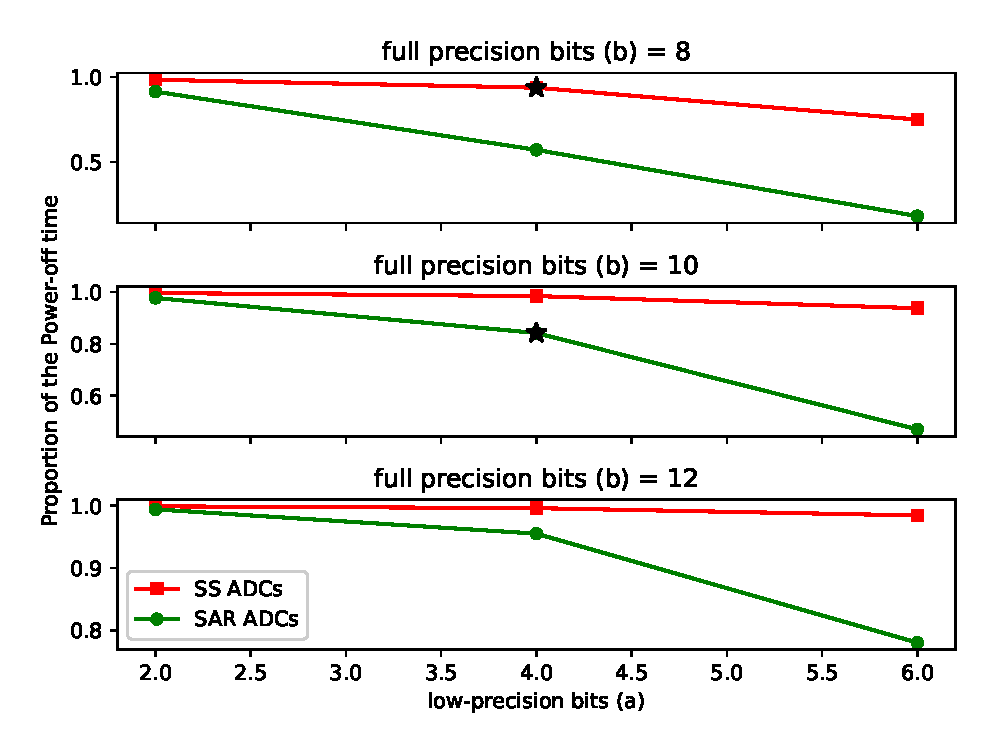
\includegraphics[width=3.5in]{./Figures/Proportion.eps}}
	%\caption{Achievable Proportion of the Power-off time for the SS and SAR/SS ADCs.}
	%\label{Proportion}
%\end{figure} 

%For other different precision configurations and number of parallel columns, 
%the corresponding power consumption and energy-saving performance can also be estimated by extending the evaluation results in Sect.~\ref{result}.
